\chapter{Řízení modelu auta}
\label{sec:PlatformControl}\

V~této kapitole je popsán způsob manuálního a~automatického řízení. Pro automatické
řízení je popsán způsob rozpoznání dráhy a~řízení servo i~motorů. Pro manuální
řízení je popsán způsob ovládaní auta pomocí RC ovladače. Přepínáni mezi režimy
bylo implementováno pomocí tlačítka A~na POLI-TFC.


\section{Dráha}\

Testování řízení platformy bylo provedeno na dráze ve tvaru čísla 8.

Dráha je zobrazena na obrázku \ref{fig:Road}.

\begin{figure}[!h]
    \centering
    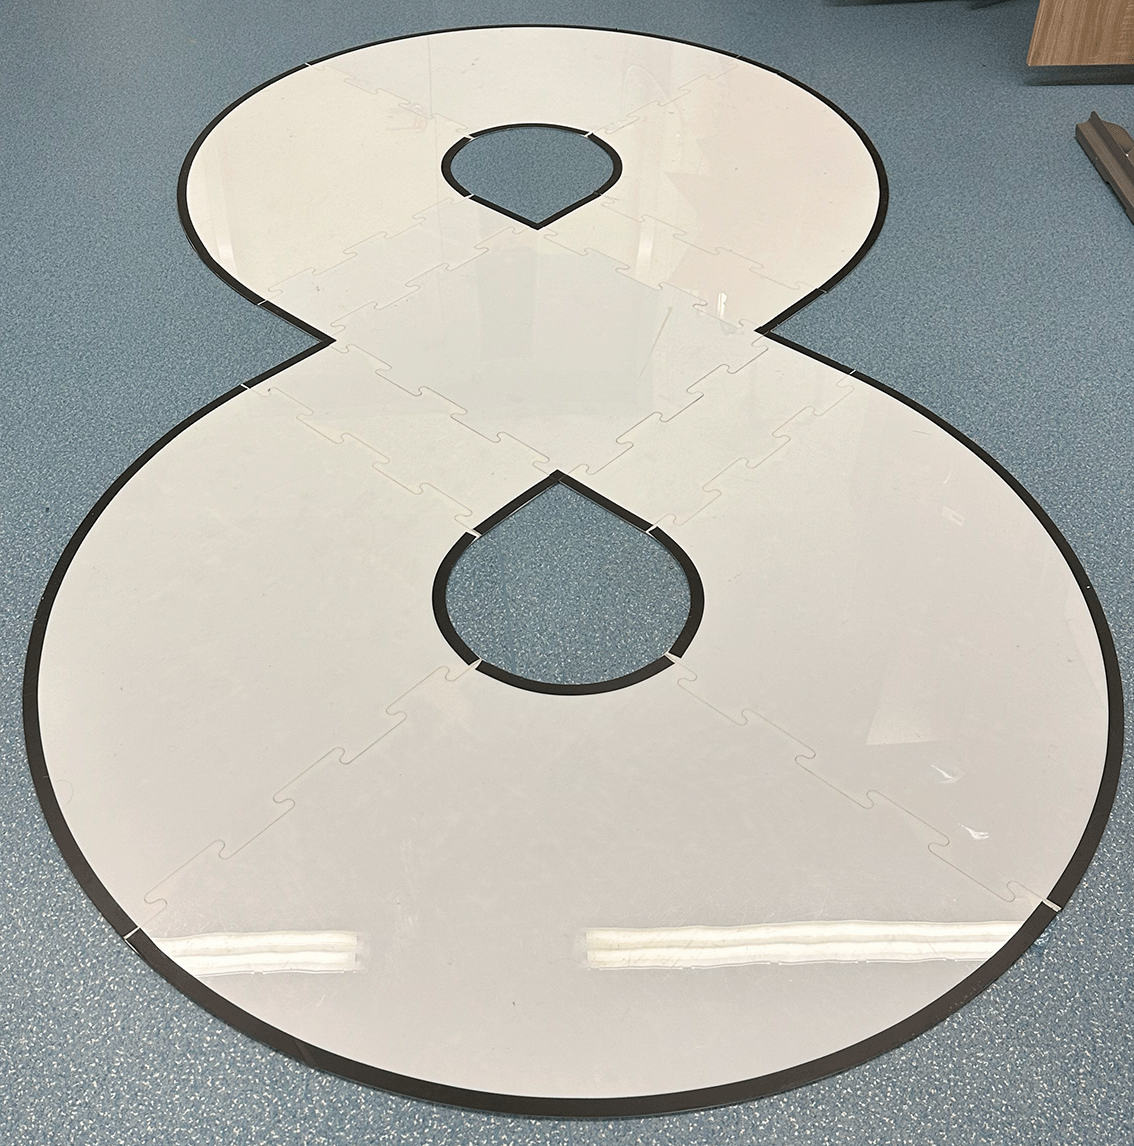
\includegraphics[width = .55\linewidth]{Figures/Road.png}
    \caption{Dráha.}
    \label{fig:Road}
    \vspace{-15pt}
\end{figure}

\section{Automatické řízení}\

\textbf{Automatické řízení} se skládá ze dvou častí. První je algoritmus rozpoznání 
drahý pomocí řádkové kamery. Druhá je kontrola motoru a~servo na základě těchto dat. 
Implementace řízení je inspirovaná bakalářskou práce Zvonka Richarda \uv{Mechanizmy 
řízení robotického auta NXP (FREESCALE)} \cite{robot}.

\subsection{Rozpoznání dráhy}\

Nejprve bylo zapotřebí získat obraz, který zajišťuje řádková kamera. Pro formát dat
je použita třída TFC \cite{draha}, která vrací data ve formátu 1D pole typu 
uint16\_t (16bitové celá čísla bez znaménka) v~intervalu <0; 4095>.

Obraz se zpracovává v~následujících krocích:
\begin{enumerate}
    \item Filtrování mediánem;
    \item Normalizace obrazu;
    \item Prahování průměrem.
\end{enumerate}

\subsubsection*{Filtrování mediánem}\

\textbf{Filtrování mediánem} je užitečné pro odstranění malých artefaktů v~obraze.
Zpracování pixelů probíhá na základě jeho okolních pixelů. Je zapotřebí tak mít
uloženy všechny pixely. Každá hodnota pixelu je nahrazena mediánem hodnot v~určitém
okolí daného pixelu, což pomáhá zachovat ostré hrany obrazu, zatímco šum je
redukován. Ukázka použitého algoritmu je ve výpisu \ref{lst:slowMedianBlur} 
\cite{draha}\cite{robot}.

\begin{lstlisting}[caption = Filtrování mediánem., label = lst:slowMedianBlur]
void Image::fastMedianBlur(RefCImageLine srcImg, RefImageLine dstImg,
                           int pixels) {
    memcpy(dstImg, srcImg, LINE_LENGTH);
   
    const int buffSize = pixels * 2 + 1;
    std::vector<uint16_t> blurBuffer;

    for (int i~= ((LINE_LENGTH / 2) % pixels) + pixels;
         i~< LINE_LENGTH - pixels; i~+= buffSize) {
        
        for (int j = -pixels; j <= pixels; j++) {
            blurBuffer.emplace_back(srcImg[i + j]);
        }
        
        std::sort(blurBuffer.begin(), blurBuffer.end());
        for (int j = -pixels; j <= pixels; j++) {
            dstImg[i + j] = blurBuffer.at(pixels + 1);
        }
        
        blurBuffer.clear();
    }
}
\end{lstlisting}

\subsubsection*{Normalizace obrazu}\

\textbf{Normalizace obrazu} probíhá na základě nalezení minimálního a~maximálního
bodu v~celém obraze. Každý bod je normalizován v~intervalu <min; max> do intervalu
<0; 255>. 
Díky normalizaci obrazu je auto schopno se přizpůsobit k~různým  podmínkám. Použitý
algoritmus normalizace je ve výpisu \ref{lst:normalize} \cite{robot}.
\begin{lstlisting}[caption = Normalizace obrazu., label = lst:normalize]
void Image::normalize(RefCImageLine srcImg, RefImageLine dstImg) const {
    for (int i~= 0; i~< LINE_LENGTH; i++) {
        auto pixel = static_cast<float>(srcImg[i]);
        pixel -= this->minValue;
        pixel *= COLOR_WHITE;
        pixel /= (this->maxValue - this->minValue);
        dstImg[i] = static_cast<uint16_t>(pixel);
    }
}
\end{lstlisting}

\subsubsection*{Prahování průměrem}\

Pomocí prahování se obraz převádí do binárního formátu (formát, který se skládá
pouze ze~dvou hodnot (0, 1)). Zapotřebí je tak určit hodnotu prahu pro každý pixel.
Pokud pixel je nižší než práh, je nastaven na 0, jinak je nastaven na 1 nebo 255.
Ukázku algoritmu je ve výpisu \ref{lst:threshold} \cite{robot}.
\begin{lstlisting}[caption = Prahování průměrem., label = lst:threshold]
void Image::threshold(RefCImageLine srcImg, RefImageLine dstImg) const {
    for (int i~= 0; i~< LINE_LENGTH; i++) {
        if (srcImg[i] < this->threshValue)
            dstImg[i] = COLOR_BLACK;
        else
            dstImg[i] = COLOR_WHITE;
    }
}
\end{lstlisting}

Pro získání hodnoty prahu byla použit vzorec:
\begin{align}
y = \frac{1}{N} \sum_{i = 0}^{N}x[i],
\end{align}
kde $y$ je výsledná hodnota práhu, $N$ je šířka obrazu a~$x[i]$ je hodnota pixelu. Hodnota $N$ je 128, dle rozměru pole získaného z~řádkové kamery. 

\subsection{Řízení servomotoru}\
\label{sec:servocontrol}

Pro řízení pozice servomotoru je použit \textbf{PID regulátor}. PID reguluje
zařízení tak, aby odchylka byla od nastavené hodnoty co nejmenší. Skládá se ze 3
složek: proporcionální, integrační, derivační~\cite{PID}.

Pro proporcionální složku se používá rozdíl poměru vzdálenosti čar od okrajů obrazu.
\begin{lstlisting}[caption = Kalkulace poměru vzdálenosti čar., label = lst:calculateDistanceRatio]
float Core::calculateDistanceRatio() {
    this->tracer.addImage(data.line);
    std::pair<uint8_t, uint8_t> distances = tracer.getDistancesPair();
    data.leftDistance = distances.first;
    data.rightDistance = Shared::Image::LINE_LENGTH - distances.second;
    const float leftRatio = static_cast<float>(data.leftDistance) /
                            static_cast<float>(data.rightDistance);
    const float rightRatio = static_cast<float>(data.rightDistance) /
                             static_cast<float>(data.leftDistance);
    data.regionsCount =
        tracer.getRegions(data.line, 0, TFC_CAMERA_LINE_LENGTH - 1, false).size();
    data.regionsListSize = tracer.listSize_;
    data.unchangedLeft = tracer.unchangedLeft_;
    data.unchangedRight = tracer.unchangedRight_;
    data.hasLeft = tracer.hasLeft_;
    data.hasRight = tracer.hasRight_;
    return rightRatio - leftRatio;
}
\end{lstlisting}

Hledaní těchto čar je implementováno pomocí algoritmu pod názvem \uv{Hledání
Regionu}. Region je struktura, která uchovává indexy okrajů oblastí jedné barvy.
Algoritmus hledá regiony ve smyčce, která si uchovává barvy a~porovná je s~barvou
samotného bodu. Jestliže se barva změnila, znamená to konec jednoho regionu
a~začátek nového. Zmíněný algoritmus je zobrazen ve výpisu \ref{lst:getRegions} 
\cite{robot}.

\begin{lstlisting}[caption = Algoritmus \uv{Hledání Regionu}., label = lst:getRegions]
std::vector<Shared::Region> LineTracer::getRegions(const Shared::Image &image, uint8_t searchLeftIdx, uint8_t searchRightIdx, bool saveToClass ) {
	std::vector<Shared::Region> foundRegions;
	uint8_t currentColor = static_cast<uint8_t>(image.atThresh(searchLeftIdx));
	foundRegions.emplace_back(Shared::Region({searchLeftIdx, searchLeftIdx, currentColor}));
	for (uint8_t i~= searchLeftIdx; i~<= searchRightIdx; i++) {
		if (currentColor != image.atThresh(i)) {
			if (foundRegions.size() > MAX_REGIONS_COUNT) {
				break;
			}
			foundRegions.at(foundRegions.size() - 1).right = i;
			foundRegions.emplace_back(Shared::Region({i, i, image.atThresh(i)}));
		}
		currentColor = static_cast<uint8_t>(image.atThresh(i));
	}
	if(saveToClass){
		currentRegions_ = foundRegions;
	}
	return foundRegions;
}
\end{lstlisting}

\subsection{PWM řízení motorů}\

U~řízení motorů musíme rozlišovat dvě fáze: \textbf{zatáčení} a~\textbf{jízdu
rovně}. Pro rozpoznaní fázi zatáčení je použit algoritmus mediánu historie obrazu.
Aplikace si uchovává historii zpracovaných záznamů (regionů) a~pro oba okraje je
vypočítán medián. Pokud se okraje aktuálního řídícího regionu nachází v~blízkém
okolí vypočteného mediánu, auto se pravděpodobně nachází na rovině a~oba motory se
mohou otáčet na maximálně nastavený výkon. Pokud jinak, auto se pravděpodobně
nachází v~zatáčce a~je tedy potřeba zpomalit motor na straně, kde se nachází okraj.
Zpomalení je implementováno na základě úhlu servomotoru. Algoritmus je ve výpisu 
\ref{lst:getRegions} \cite{robot}.

\begin{lstlisting}[caption = Algoritmus kontroly PWM motorů., label = lst:controlPWM]
float speed = SPEED;
data.angle = (data.servoPosition * 5.85f / 200) * PI /
	                 180.f; // Convert servo to angle
if (!(this->tracer.unchangedLeft_ && this->tracer.unchangedRight_)) {
    innerSpeed =
        speed * (1.f - DIFF_COEF * (1.50f * tanf(data.angle)) / 2.f * 1.85f);
    outerSpeed =
        speed * (1.f + DIFF_COEF * (1.50f * tanf(data.angle)) / 2.f * 1.85f);
    if (data.angle > 0.f) {
        data.rightSpeed = innerSpeed;
        data.leftSpeed = outerSpeed;
    } else {
        data.leftSpeed = innerSpeed;
        data.rightSpeed = outerSpeed;
    }
    data.servoPosition *= 1.5f;
    data.leftSpeed *= 0.75f;
    data.rightSpeed *= 0.75f;
} else {
    data.leftSpeed = speed;
    data.rightSpeed = speed;
}
\end{lstlisting}

\section{Manuální řízení}\

Pro manuální řízení byl použit \textbf{vysílač HITEC OPTIC 6 SPORT}.
Vysílač je zobrazen na~obrázku \ref{fig:Joystick}. HITEC OPTIC 6 SPORT 
posílá signál do přijímače Minima 6S. Oba pracují na~frekvenci 2,4~GHz. 
Ovladač má dvě páky. Jedna je použitá pro zvětšení a~zmenšení
plynu motoru. Druhá je použitá pro změnu pozice servomotoru \cite{RC}.

Oba signály jsou přijímány přes kanály CH1 a~CH2 \cite{RC}. Tyto kanály jsou
integrovány do modulu POLI-TFC shield, kde jsou signály zpracovány programově
prostřednictvím třídy TFC \cite{draha}. Hodnoty signálů se nacházejí v~rozsahu
<1000; 2000>, Tyto hodnoty jsou následně transformovány do rozsahu <-1; 1> pomocí 
vzorce:

\begin{equation}
	\centering
	y = (x / 100 - 15) / 10,
\end{equation}
kde $y$ je normalizovaná hodnota a~$x$ je hodnota z~přijímače. 

Poté je $y$ násoben na maximální hodnotu PWM motorů nebo servomotoru. Výsledek je 
následně použit pro jejich nastavení.

\begin{figure}[!h]
    \centering
    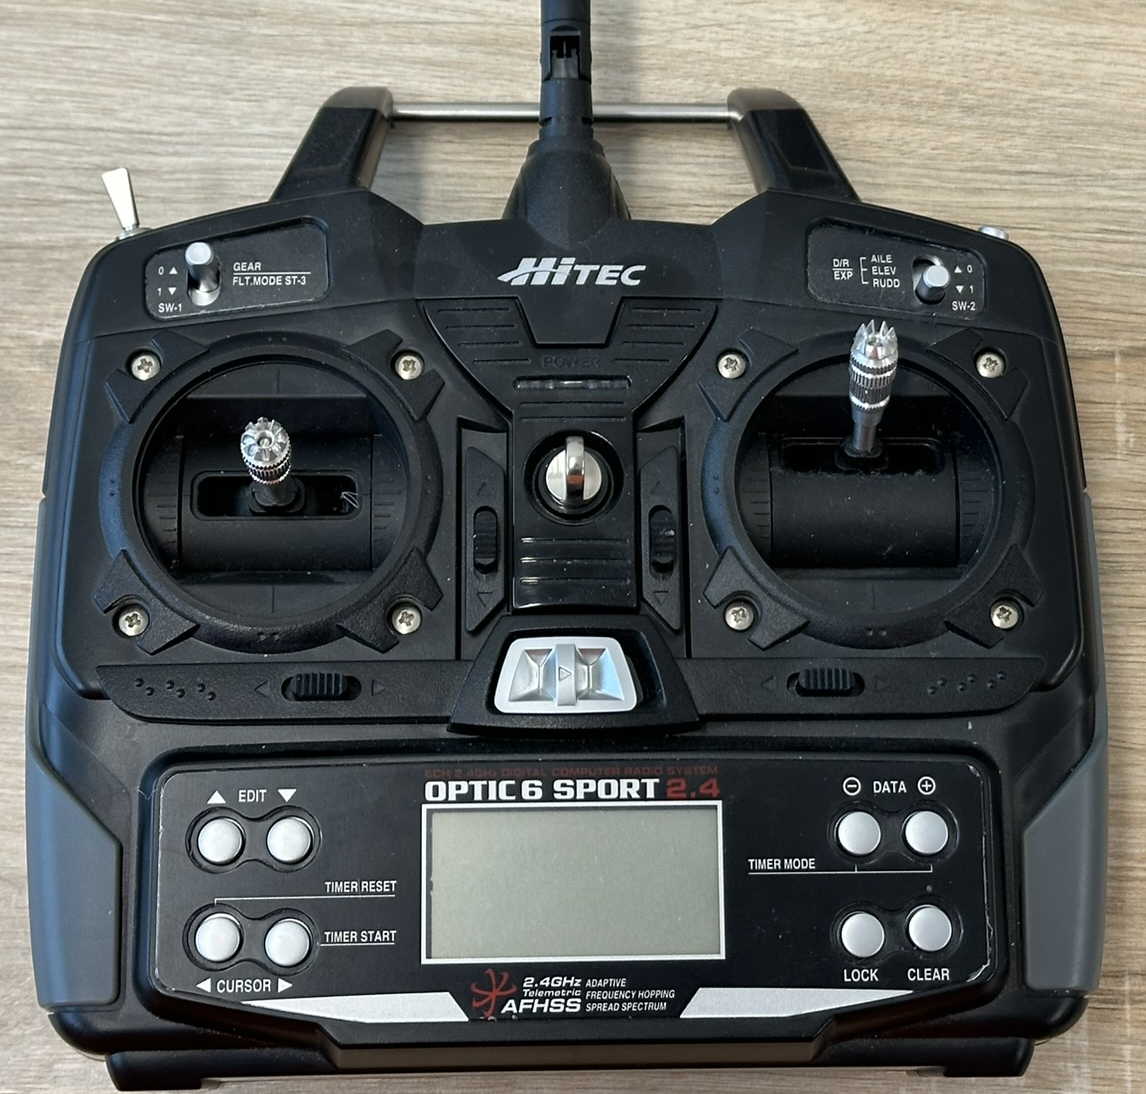
\includegraphics[width = .5\linewidth]{Figures/Joystick.png}
    \caption{Ovladač HITEC OPTIC 6 SPORT.}
    \label{fig:Joystick}
    \vspace{-10pt}
\end{figure}

\endinput